% begin module limit-ex4
\begin{frame}
\begin{example} %[Example 4, p. 98]
\begin{columns}[c]
\column{.4\textwidth}
\begin{itemize}
\item  Guess the value of $\lim_{x\rightarrow 0}\sin\frac{\pi}{x}$.
\item<2->  Notice that $\sin\frac{\pi}{x}$ is not defined at $0$.
\item<3->  It is defined for values of $x$ near $0$.
\item<5->  We may guess that the limit is $0$.
\item<6->  In this case such a guess would be \alert<6>{wrong}.
\end{itemize}
\column{.6\textwidth}
\uncover<4->{
\[
\begin{array}{|r|c|r|c|}
\hline
x & f(x) & x & f(x) \\
\hline
1 & \sin \pi = 0 &
\frac{1}{2} & \sin 2\pi = 0 \\
\frac{1}{3} & \sin 3\pi = 0 &
\frac{1}{4} & \sin 4\pi = 0 \\
0.1 & \sin 10\pi = 0 &
0.01 & \sin 100\pi = 0 \\
\hline
\end{array}
\]
}

\uncover<6->{
\psset{xunit=1.1cm,yunit=1.1cm}
\begin{pspicture}(-3,-1.5)(3,1.5)
\psframe*[linecolor=white](-3, -1.5)(3.2, 1.7)
\fcAxesStandard{-3}{-1.5}{3}{1.5}
\tiny
\rput[t](1,-0.1){ $1$}
\psplot[linewidth=0.3pt, linecolor=red, plotpoints=10000]{-3}{-0.01}{3.14159 x div 57.295779513 mul sin}
\psplot[linewidth=0.3pt, linecolor=red, plotpoints=10000]{0.01}{3}{3.14159 x div 57.295779513 mul sin}
%\pscircle*[fillcolor=white, linecolor=red](0, 1){0.07}
%\pscircle*[fillcolor=white, linecolor=white](0, 1){0.04}

\end{pspicture}
%\ 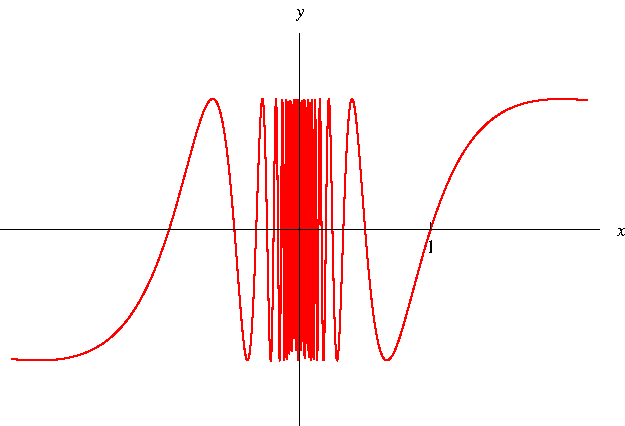
\includegraphics[height=4cm]{limits/pictures/02-01-ex4.pdf}%
}
\end{columns}
\end{example}
\end{frame}
% end module limit-ex4
